
% use pdflatex -shell-escape slides.tex to compile
\documentclass[10pt]{beamer}
\usetheme[
%%% options passed to the outer theme
%    shownavsym          % show the navigation symbols
]{AAUsimple}
  
% If you want to change the colors of the various elements in the theme, edit and uncomment the following lines
% Change the bar and sidebar colors:
%\setbeamercolor{AAUsimple}{fg=red!20,bg=red}
%\setbeamercolor{sidebar}{bg=red!20}
% Change the color of the structural elements:
%\setbeamercolor{structure}{fg=red}
% Change the frame title text color:
%\setbeamercolor{frametitle}{fg=blue}
% Change the normal text color background:
%\setbeamercolor{normal text}{fg=black,bg=gray!10}
% ... and you can of course change a lot more - see the beamer user
% manual.
\usepackage{animate}
\usepackage{tabularx}
\usepackage{epstopdf}
\usepackage{movie15}
\usepackage[utf8]{inputenc}
\usepackage[english]{babel}
%\usepackage[T1]{fontenc}
% Or whatever. Note that the encoding and the font should match. If T1
% does not look nice, try deleting the line with the fontenc.
\usepackage{helvet}
\usepackage[helvet]{sfmath}

% For math font script
\usepackage[mathscr]{euscript}

\usepackage{color, xcolor}
\usepackage{tikz}
% tikz setup for descendant robot motion figure 
\usetikzlibrary{positioning,chains,fit,shapes,calc}
\usetikzlibrary{arrows,shadows,trees}
\tikzset{
  basic/.style  = {draw, text width=2cm, drop shadow, font=\sffamily, rectangle},
  root/.style   = {basic, rounded corners=2pt, thin, align=center,
                   fill=red!30},
  level 2/.style = {basic, rounded corners=6pt, thin,align=center, fill=orange!30,
                   text width=8em},
  level 3/.style = {basic, thin, align=left, fill=pink!60, text width=8em}
}
% tikz setup for lattice graph
\usepackage{pgf}
\usetikzlibrary{automata}
\usepackage{hyperref}
\hypersetup{pdfpagemode=FullScreen}
\usepackage{ifthen}
% tikz animation
\usetikzlibrary{arrows,decorations.pathmorphing,through,backgrounds,positioning,fit,petri}
\usetikzlibrary{shapes.multipart}
\usetikzlibrary{decorations.pathreplacing}

\usepackage[tikz]{bclogo}

\newcommand{\id}{{\rm id}}
\newcommand{\edge}[3]{{#1}\overset{#2}{\longrightarrow}{#3}}
\renewcommand{\L}{{\Lambda}}
% colored hyperlinks
\newcommand{\chref}[2]{%
  \href{#1}{{\usebeamercolor[bg]{AAUsimple}#2}}%
}

\title{Constrained Geometric Approximation Approach for Robot Planning and
  Decentralized Formation Algorithm for Multi-Robot Systems}

%\subtitle{v.\ 1.0.0}  % could also be a conference name
%\date{\today}
\author{
  \underline{Yang Song}, Jason M. O'Kane\\
  \href{mailto:song24@email.sc.edu}{{\tt song24@email.sc.edu} \\
  \href{mailto:jokane@cse.sc.edu}{\tt jokane@cse.sc.edu}}
}

% - Give the names in the same order as they appear in the paper.
% - Use the \inst{?} command only if the authors have different
%   affiliation. See the beamer manual for an example

\institute[
%  {\includegraphics[scale=0.2]{aau_segl}}\\ %insert a company, department or university logo
  Dept.\ of Computer Science and Engineering\\
  University of South Carolina
] % optional - is placed in the bottom of the sidebar on every slide
{% is placed on the bottom of the title page
  Dept. of Computer Science and Engineering\\
  University of South Carolina
  
  %there must be an empty line above this line - otherwise some unwanted space is added between the university and the country (I do not know why;( )
}

% specify a logo on the titlepage (you can specify additional logos an include them in 
% institute command below
\pgfdeclareimage[height=1.5cm]{titlepagelogo}{sc_logo.pdf}%{aau_logo_new.pdf} % placed on the title page
%\pgfdeclareimage[height=1.5cm]{titlepagelogo2}{aau_logo_new.pdf} % placed on the title page
\titlegraphic{% is placed on the bottom of the title page
  \pgfuseimage{titlepagelogo}
%  \hspace{1cm}\pgfuseimage{titlepagelogo2}
}

\definecolor{scred}{RGB}{115,0,10}% dark red 
\definecolor{myblue}{RGB}{80,80,160}
\definecolor{mygreen}{RGB}{80,160,80}

\begin{document}
% the titlepage
\begin{frame}[plain] % the plain option removes the sidebar and header from the title page
  \titlepage
\end{frame}
%%%%%%%%%%%%%%%%
% TOC
% \begin{frame}{Agenda}{}
% \tableofcontents
% \end{frame}
%%%%%%%%%%%%%%%%
%%%%%%%%%%%%%%%%%%%%%%%%%%%%%%%%%%%%%%%%%%%%%%%%%%%%%%%%%%%%%%%%%%%%%%%%%%%%%%%%%%%%%%%%%%%%%%%%%%%%%%%
\begin{frame}
  \frametitle{Outlines}
  \tableofcontents[]
\end{frame}
\section{CGA for Robot Planning}
%\subsection[Problem]{Overview}
\begin{frame}{Constrained Geometric Approximation}
\begin{columns}
  \begin{column}{.65\textwidth}
    \begin{itemize}
    \item \textbf{Goal}:\\
    For an extremely simple robot with:
    \begin{itemize}
    \item computation limitations
    \item moving and sensing uncertainties
    \end{itemize}
    represent and reason about uncertainty in its own states efficiently.\\
    \item \textbf{Basic Idea}:\\
    Explicitly represent what the robot knows as an information state (\textit{I-state}).
    \item \textbf{Intuition}:\\
    Accelerate time-consuming operations by maintaining only an \textcolor[rgb]{1.00,0.00,0.00}{overapproximation} of the true
    \emph{I-state}, and constraining this approximation
    to have a simple geometric form.\\
    \end{itemize}
  \end{column}
  \begin{column}{.35\textwidth}
    %\textbf{Result}:\\
%    The robot can fulfill the navigation task even with poor approximation of the true \emph{I-state}.
    \begin{figure}
    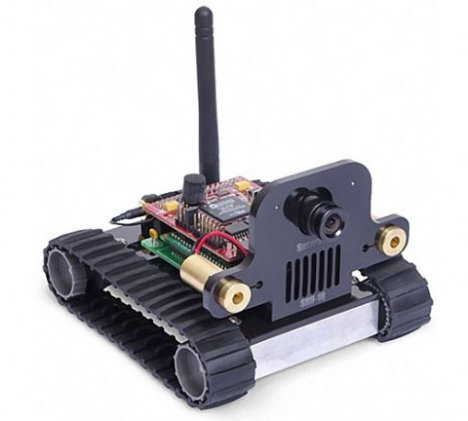
\includegraphics[scale=0.2]{figs/srvq.jpg}
    \end{figure}
    SRV-1 Surveyor Robot
  \end{column}
\end{columns}
\end{frame}

%\subsection[Problem]{Problem Statement}
\begin{frame}{Robot Model}
Assume that current real state of the robot could not be observed directly.  The
robot could maintain an \emph{I-state} $\eta_k$, to make its decisions.
\begin{itemize}
\item Robot state at stage $k$: $x_k \in X$,
\item State transition function: $F(x_k, u_k)$.
\item Robot action at stage $k$: $u_k$.
\item Information state (\emph{I-state}) at stage $k$: $\eta_k$ is a set of
  possible states at stage $k$
\end{itemize}
\begin{figure}
  \begin{tikzpicture}[scale=0.5]
    \draw[violet, fill=orange!40] (3, 3) circle (3);
    \draw[fill=blue] (3,4.5) circle (0.2);
    \draw[fill=blue] (3.2,1.7) circle (0.2);
    \draw[fill=blue] (1,3) circle (0.2);
    \draw[fill=blue] (2,0.5) circle (0.2);
    \draw[fill=blue] (4,3.3) circle (0.2);
    \draw[fill=blue] (4.4,4.8) circle (0.2);
  \end{tikzpicture}
  % 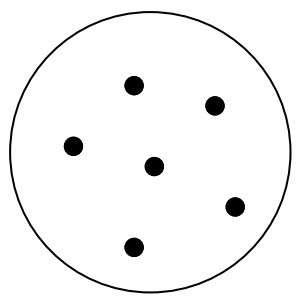
\includegraphics[scale=0.3]{figs/xk.jpg}
  \caption{I-state $\eta_k$ contains all possible states}
  \label{fig:istate}
\end{figure}
\end{frame}

\begin{frame}{Example Application}{Rectangle Approximation}
  \begin{center}
  %\href{run:/usr/local/bin/mplayer -fs videos/rect.mp4}{
  %  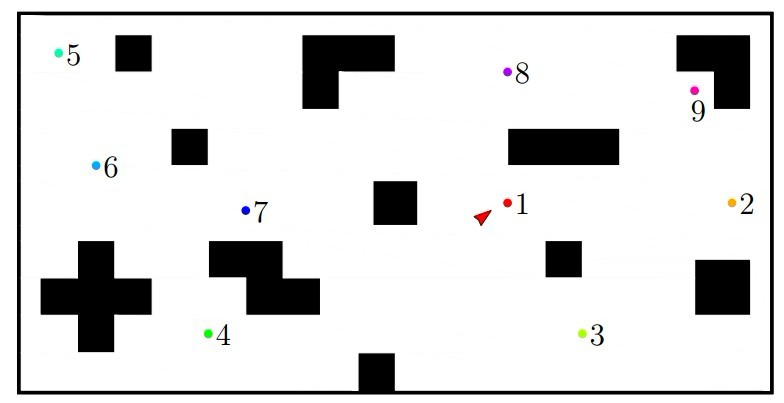
\includegraphics[scale=0.25]{figs/clutter.jpg}}
    \includemovie[toolbar,poster,autoplay]{6cm}{6cm}{videos/rect.mp4}
  \end{center}
\end{frame}


\begin{frame}{Prior Work}
\begin{itemize}
\item Prior research done by (B. Tovar and S. M. LaValle) and (J. van den Berg,
  P. Abbeel, and K. Goldberg)
  used probabilistic representations for planning\\

\item Prior work by the J.O'Kane has used preliminary versions of the
  constrained geometric approximation method using specific, fixed range spaces.
\end{itemize}
New contributions
\begin{enumerate}
\item A careful formulation of the operations in the range space $\mathcal{R}$.
\item Algorithms for double-rectangle range space $\mathcal{R}_{drect}$.
\item A series of experiments for effectiveness comparison of different range spaces.
\end{enumerate}
\end{frame}
%%%%%%%%%%%%%%%%%%%%%%%%%%%%%%%%%%%%%%%%%%%%%%%%%%%%%%%%%%%%%%%%%%%%%%%%%%%%%%%%%%%%%%%%%%%%%%%%%%%%%%%
\begin{frame}
  \frametitle{Outlines}
  \tableofcontents[]
\end{frame}
\section[Range Space]{Range Space}
%\subsection[Range Space Definition]{Range Space Definition}
\begin{frame}{Range Space}
  \begin{definition}{\textbf{A range space}}
    $\mathcal{R} \subseteq \mathcal{I}$ is a set of I-states, contains
    approximation of \emph{I-states}, $A(\eta_k) \in \mathcal{R}$, equipped with
    two operations:
  \end{definition}
  \begin{columns}
    \begin{column}{.5\textwidth}
      \begin{enumerate}
      \item An \emph{approximate observation update function} $O: \mathcal{R} \times
        Y \to \mathcal{R}$, such that if $\eta_k \subseteq A(\eta_k)$, then
        $$\eta_k \cap H(y_k) \subseteq O(A(\eta_k), u_k)$$
      \item An \emph{approximate action update function} $T: \mathcal{R} \times U \to
        \mathcal{R}$, such that if $\eta_k \subseteq A(\eta_k)$, then
        $$\bigcup_{x_k \in \eta_k} F(x_k, u_k) \subseteq T(A(\eta_k), u_k)$$
      \end{enumerate}
    \end{column}
    \begin{column}{.4\textwidth}
    \begin{figure}
      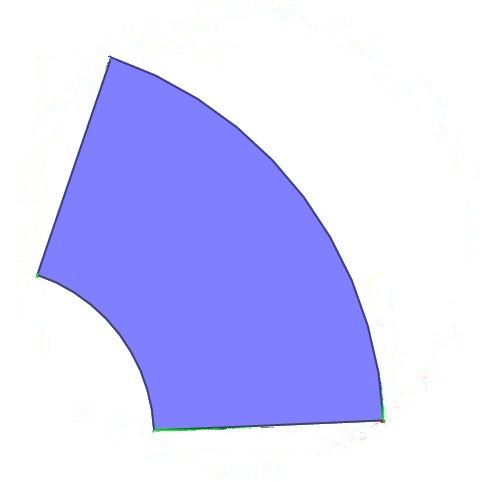
\includegraphics[scale=0.3]{figs/norangespace.jpg}
      \caption{An \emph{I-state} $\eta_k$}
    \end{figure}
  \end{column}
\end{columns}
\end{frame}

\begin{frame}{Range Space}
\begin{definition}{\textbf{A range space}}
 $\mathcal{R} \subseteq \mathcal{I}$ is a set of I-states, contains
 approximation of \emph{I-states}, $A(\eta_k) \in \mathcal{R}$, equipped with
 two operations:
\end{definition}
\begin{columns}
\begin{column}{.5\textwidth}
\begin{enumerate}
\item An \emph{approximate observation update function} $O: \mathcal{R} \times
		Y \to \mathcal{R}$, such that if $\eta_k \subseteq A(\eta_k)$, then
			$$\eta_k \cap H(y_k) \subseteq O(A(\eta_k), u_k)$$
\item An \emph{approximate action update function} $T: \mathcal{R} \times U \to
		\mathcal{R}$, such that if $\eta_k \subseteq A(\eta_k)$, then
			$$\bigcup_{x_k \in \eta_k} F(x_k, u_k) \subseteq T(A(\eta_k), u_k)$$
\end{enumerate}
\end{column}
\begin{column}{.4\textwidth}
  \begin{figure}
    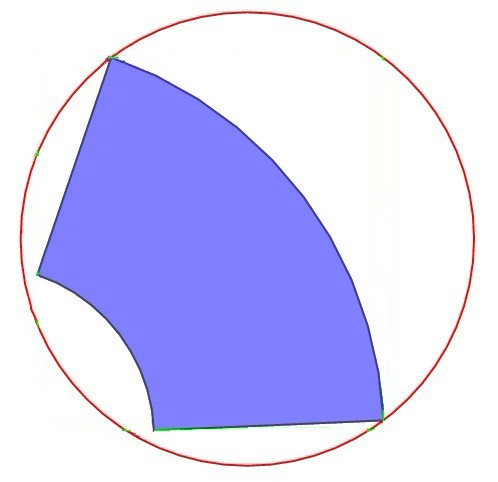
\includegraphics[scale=0.3]{figs/rangespace_circle.jpg}
    \caption{Disk overapproximation $A(\eta_k) \in \mathcal{R}_{disk}$ in red.}
    \end{figure}
\end{column}
\end{columns}
\end{frame}

\begin{frame}{Range Space}
\begin{definition}{\textbf{A range space}}
 $\mathcal{R} \subseteq \mathcal{I}$ is a set of I-states, contains
 approximation of \emph{I-states}, $A(\eta_k) \in \mathcal{R}$, equipped with
 two operations:
\end{definition}
\begin{columns}
\begin{column}{.5\textwidth}
\begin{enumerate}
\item An \emph{approximate observation update function} $O: \mathcal{R} \times
		Y \to \mathcal{R}$, such that if $\eta_k \subseteq A(\eta_k)$, then
			$$\eta_k \cap H(y_k) \subseteq O(A(\eta_k), u_k)$$
\item An \emph{approximate action update function} $T: \mathcal{R} \times U \to
		\mathcal{R}$, such that if $\eta_k \subseteq A(\eta_k)$, then
			$$\bigcup_{x_k \in \eta_k} F(x_k, u_k) \subseteq T(A(\eta_k), u_k)$$
\end{enumerate}
\end{column}
\begin{column}{.4\textwidth}
  \begin{figure}
    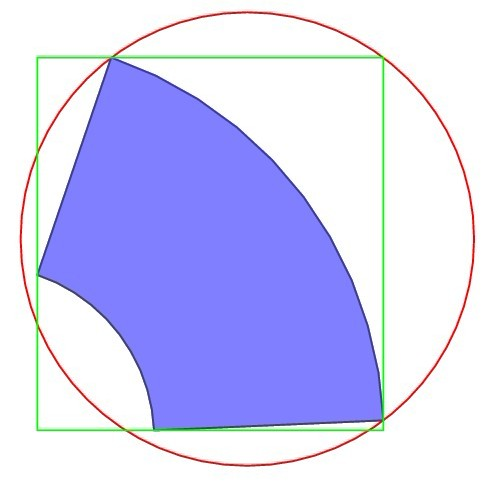
\includegraphics[scale=0.3]{figs/rangespace.jpg}
    \caption{Rectangle overapproximation $A(\eta_k) \in \mathcal{R}_{rect}$.}
  \end{figure}
\end{column}
\end{columns}
\end{frame}


\subsection[Disk Range Space]{Disk Range Space}
\begin{frame}{Observation Update in $\mathcal{R}_{disk}$}
  Approximated I-state $A(\eta_k) \in \mathcal{R}_{disk}$, where $x_k$ denotes
  the real state but unknown to robot.
			
    \begin{figure}
    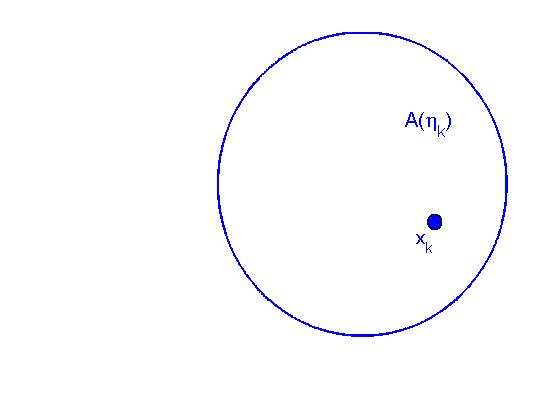
\includegraphics[scale=0.3]{figs/circle1_2.jpg}
    \end{figure}
 
\end{frame}

\begin{frame}{Observation Update in  $\mathcal{R}_{disk}$}
  Approximated I-state $A(\eta_k) \in \mathcal{R}_{disk}$ intersects with
  observation preimage $H(y_k)$ .
			
    \begin{figure}
    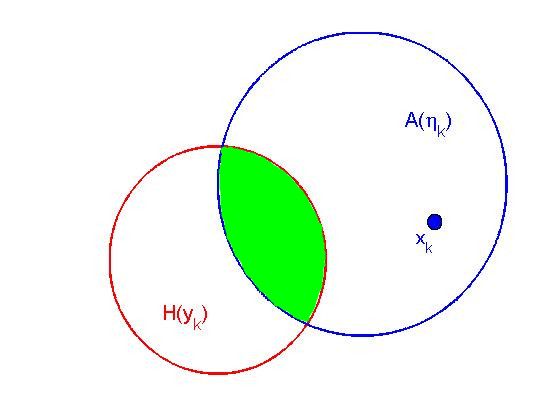
\includegraphics[scale=0.3]{figs/circle2_2.jpg}
    \end{figure}
 		
\end{frame}

\begin{frame}{Observation Update in $\mathcal{R}_{disk}$}
  The green region of intersection is the updated I-state $\eta_{k+1}$, and the
  green disk is the approximation $A(\eta_{k+1})$ of $\eta_{k+1}$.
			
    \begin{figure}
    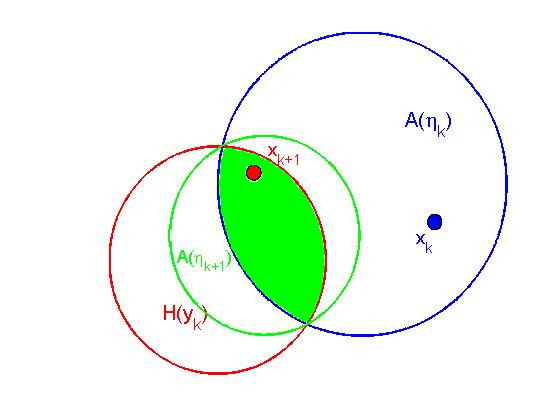
\includegraphics[scale=0.3]{figs/circle3_2.jpg}
    \end{figure}
 
\end{frame}

\begin{frame}{Observation Update in $\mathcal{R}_{rect}$}
\begin{definition}{\textbf{$AABB(S)$} :}
    For any compact set $S \subset \mathbb{R}^2$, let $AABB(S)$
	denote the its smallest	``axis-aligned bounding box.''
\end{definition}

In $\mathcal{R}_{rect}$, computing approximate observation update function $O_{rect}$ takes $O(1)$ time:\\
$$ O_{rect}(A_k, y_k) = AABB(H(y_k) \cap A(\eta_k)), A_k = A(\eta_k) \in \mathcal{R}_{rect}$$

\begin{figure}
    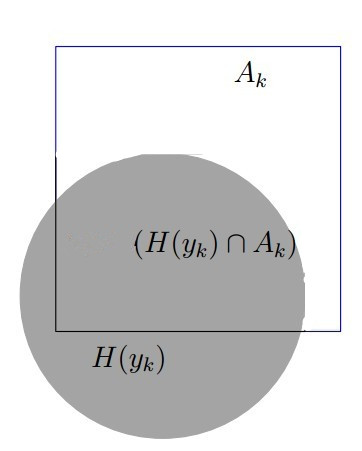
\includegraphics[scale=0.27]{figs/circlerect_1.jpg}
    \end{figure}
 
\end{frame}

\subsection[Rectangle Range Space]{Rectangle Range Space}
\begin{frame}{Observation Update in $\mathcal{R}_{rect}$}
  \begin{definition}{\textbf{$AABB(S)$} :}
    For any compact set $S \subset \mathbb{R}^2$, let $AABB(S)$ denote the its
    smallest ``axis-aligned bounding box.''
  \end{definition}

  In $\mathcal{R}_{rect}$, computing approximate observation update function $O_{rect}$ takes $O(1)$ time:\\
  $$ O_{rect}(A_k, y_k) = AABB(H(y_k) \cap A(\eta_k)), A_k = A(\eta_k) \in \mathcal{R}_{rect}$$
  \begin{figure}
    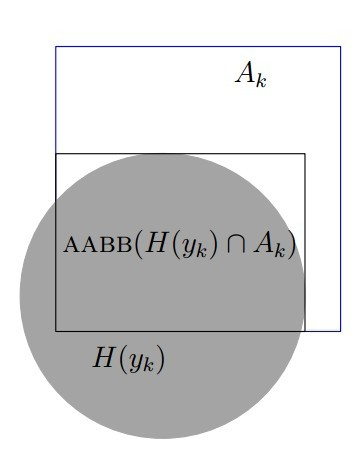
\includegraphics[scale=0.27]{figs/circlerect.jpg}
  \end{figure}
\end{frame}

\begin{frame} {Action Update in $\mathcal{R}_{rect}$}
  In $\mathcal{R}_{rect}$, computing approximate action update function $T_{rect} :$\\
  $$T_{rect}(A(\eta_k), u_k) = AABB(X_{free} \cap [A(\eta_k) \oplus \{ u_k \} \oplus AABB(\Theta(u_k))])$$
  \begin{figure}
    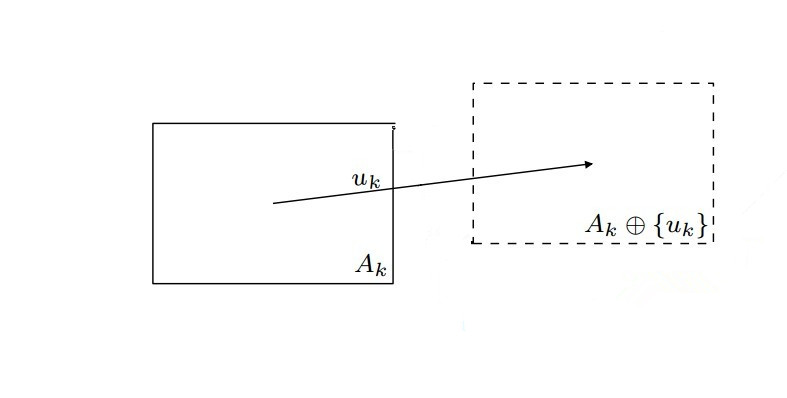
\includegraphics[scale=0.35]{figs/t_rect.jpg}
    \caption{Transition of $A(\eta_k)$ given action $u_k$, $\oplus$ is Minkowski addition of two sets.}
  \end{figure}
\end{frame}

\begin{frame}{Action Update in $\mathcal{R}_{rect}$}
  In $\mathcal{R}_{rect}$, computing approximate action update function $T_{rect} :$\\
  $$T_{rect}(A(\eta_k), u_k) = AABB(X_{free} \cap [A(\eta_k) \oplus \{ u_k \} \oplus AABB(\Theta(u_k))])$$
  \begin{figure}
    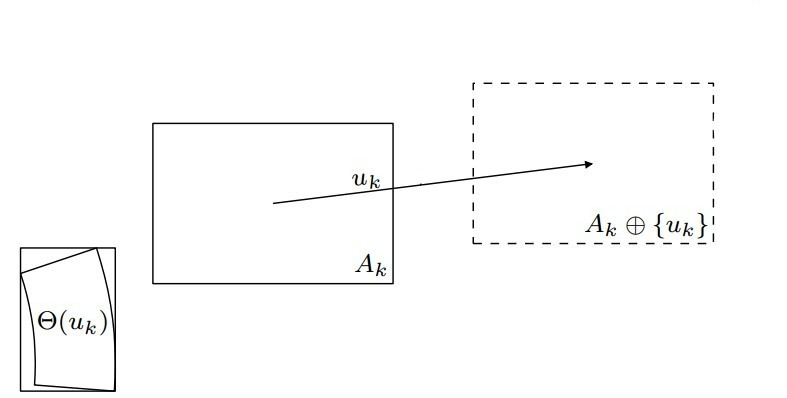
\includegraphics[scale=0.35]{figs/t_rect2.jpg}
    \caption{Consider approximation of the bounded motion uncertainty $\Theta(u_k)$.}
  \end{figure}
\end{frame}

\begin{frame}{Action Update in $\mathcal{R}_{rect}$}
  In $\mathcal{R}_{rect}$, computing approximate action update function $T_{rect} :$\\
  $$T_{rect}(A(\eta_k), u_k) = AABB(X_{free} \cap [A(\eta_k) \oplus \{ u_k \} \oplus AABB(\Theta(u_k))])$$
  \begin{figure}
    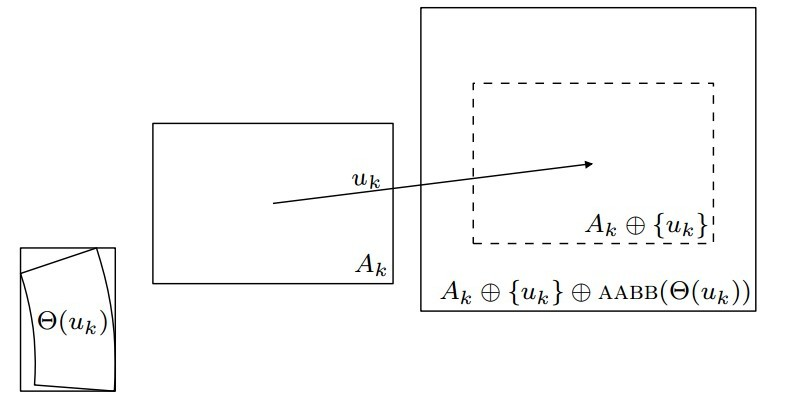
\includegraphics[scale=0.35]{figs/step12.jpg}
    \caption{Find Minkowski sum of bounded noise and approximation transition}
  \end{figure}
\end{frame}


\begin{frame}{Action Update in $\mathcal{R}_{rect}$}
  In $\mathcal{R}_{rect}$, computing approximate action update function $T_{rect} :$\\
  $$T_{rect}(A(\eta_k), u_k) = AABB(X_{free} \cap [A(\eta_k) \oplus \{ u_k \} \oplus AABB(\Theta(u_k))])$$
  \begin{figure}
    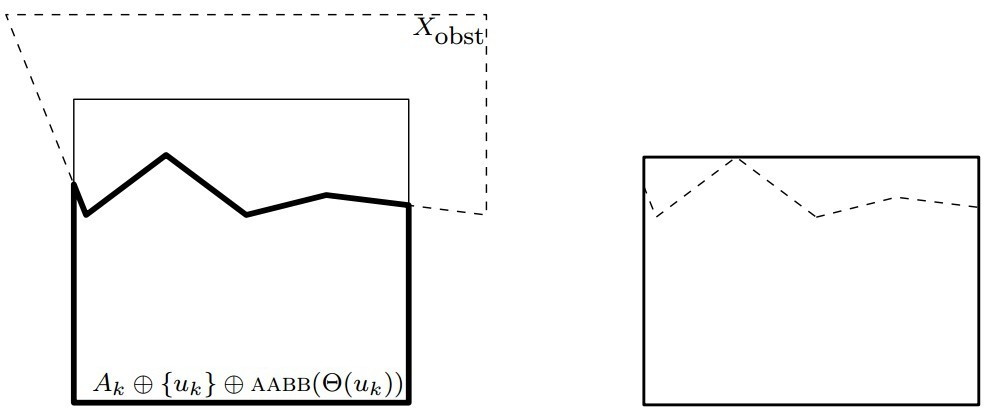
\includegraphics[scale=0.35]{figs/step34.jpg}
    \caption{If there is obstacles, intersect with $X_{free}$ first and
      then find the bounding box of the intersection.}
  \end{figure} 
\end{frame}

\subsection[Double-Rectangle Range Space]{Double-Rectangle Range Space}
\begin{frame}{Double-Rectangle approximated I-state}
  \begin{itemize}
  \item For better overapproximation quality for non-convex \emph{I-states},
    we proposed a more expressive range space of \emph{double rectangles}: \\
    \begin{equation}
      \mathcal{R}_{drect} = \{ R_1 \cup R_2 \mid R_1, R_2 \in \mathcal{R}_{rect} \}
    \end{equation}
  \item Aims to improve the approximation quality.
    \begin{figure}
      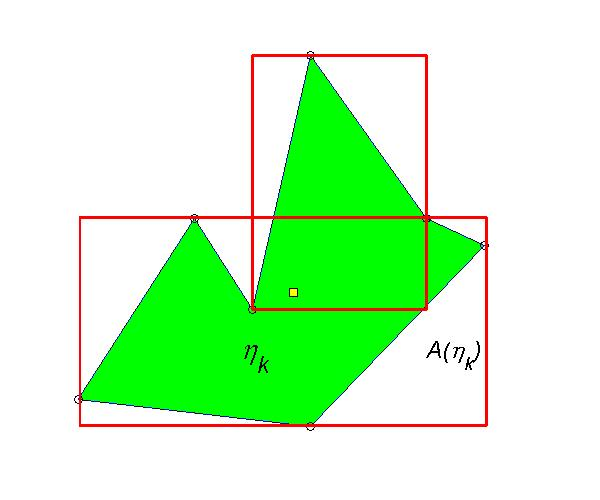
\includegraphics[scale=0.2]{figs/poly.jpg}
      %\caption{Non-convex \emph{I-state}}
    \end{figure}
  \end{itemize}
\end{frame}
\begin{frame}{DRAP Algorithm}
  ``Double Rectangle Around Polygon'' (\textbf{DRAP}) algorithm:\\
  \begin{itemize}
  \item input is a $n$-edge polygonal region of the plane
  \item output is a small double rectangle containing that polygon
  \item run time: $O(n^3)$
  \end{itemize}
  \begin{figure}
    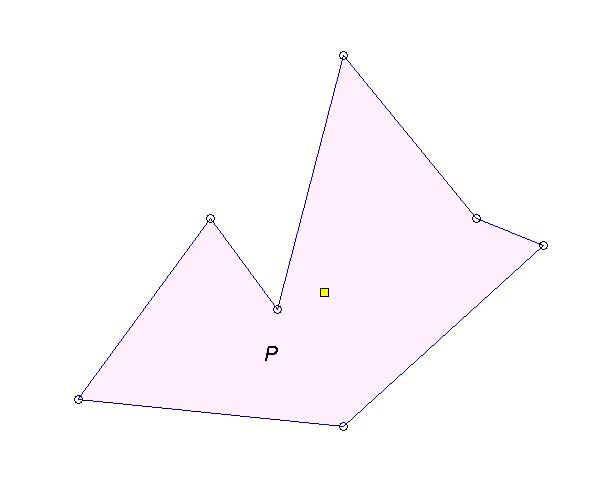
\includegraphics[scale=0.3]{figs/drapP.jpg}
  \end{figure}
\end{frame}

\begin{frame} {DRAP Algorithm}
  ``Double Rectangle Around Polygon'' (\textbf{DRAP}) algorithm:\\
  \begin{itemize}
  \item input is a $n$-edge polygonal region of the plane
  \item output is a small double rectangle containing that polygon
  \item run time: $O(n^3)$
  \end{itemize}
  \begin{figure}
    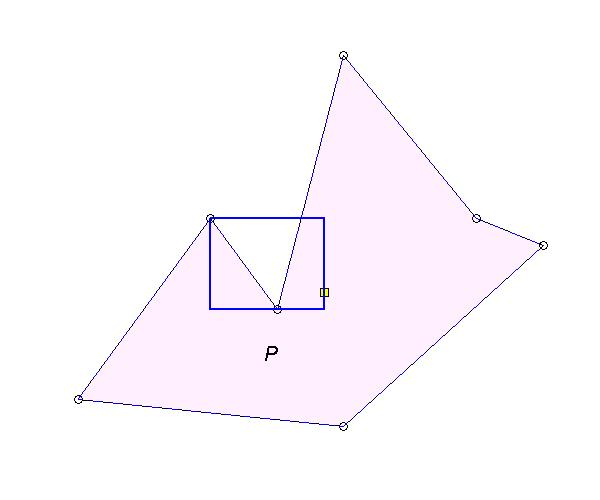
\includegraphics[scale=0.3]{figs/drap1.jpg}
  \end{figure}
\end{frame}

\begin{frame}{DRAP Algorithm}
  ``Double Rectangle Around Polygon'' (\textbf{DRAP}) algorithm:\\
  \begin{itemize}
  \item input is a $n$-edge polygonal region of the plane
  \item output is a small double rectangle containing that polygon
  \item run time: $O(n^3)$
  \end{itemize}
  \begin{figure}
    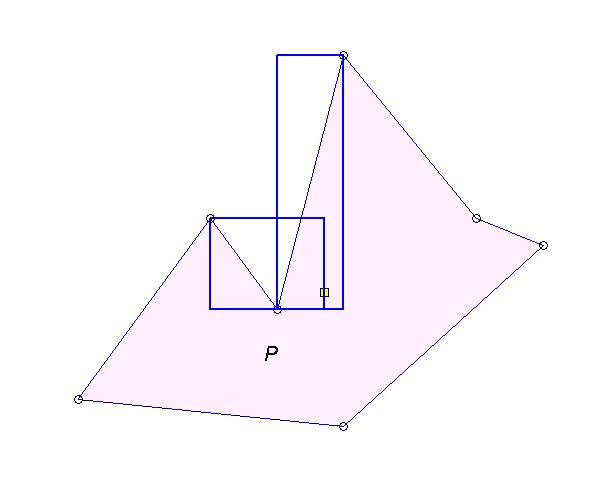
\includegraphics[scale=0.3]{figs/drap2.jpg}
  \end{figure} 
\end{frame}


\begin{frame}{DRAP Algorithm}
  ``Double Rectangle Around Polygon'' (\textbf{DRAP}) algorithm:\\
  \begin{itemize}
  \item input is a $n$-edge polygonal region of the plane
  \item output is a small double rectangle containing that polygon
  \item run time: $O(n^3)$
  \end{itemize}
  \begin{figure}
    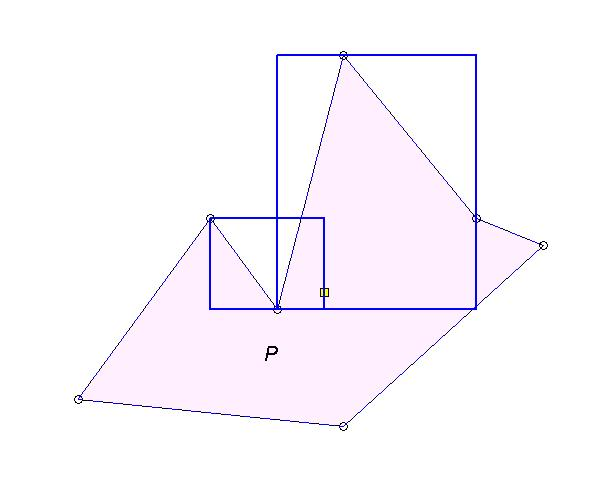
\includegraphics[scale=0.3]{figs/drap3.jpg}
  \end{figure}
\end{frame}

\begin{frame}{DRAP Algorithm}
  ``Double Rectangle Around Polygon'' (\textbf{DRAP}) algorithm:\\
  \begin{itemize}
  \item input is a $n$-edge polygonal region of the plane
  \item output is a small double rectangle containing that polygon
  \item run time: $O(n^3)$
  \end{itemize}
  \begin{figure}
    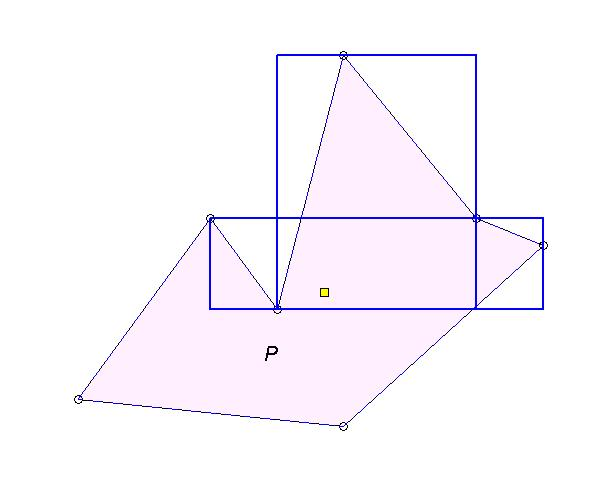
\includegraphics[scale=0.3]{figs/drap4.jpg}
  \end{figure}
\end{frame}

\begin{frame}{DRAP Algorithm}
  ``Double Rectangle Around Polygon'' (\textbf{DRAP}) algorithm:\\
  \begin{itemize}
  \item input is a $n$-edge polygonal region of the plane
  \item output is a small double rectangle containing that polygon
  \item run time: $O(n^3)$
  \end{itemize}
  \begin{figure}
    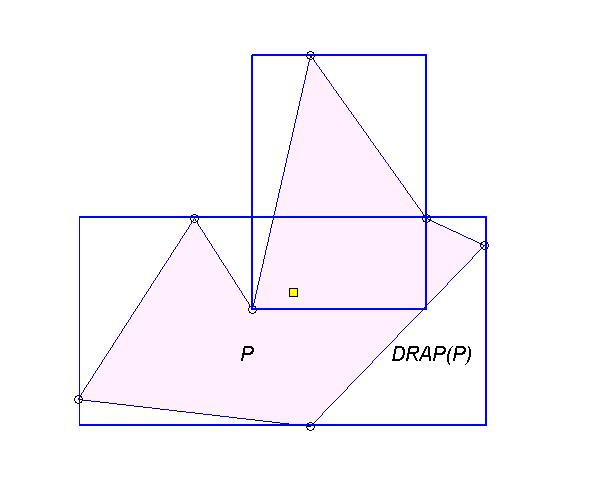
\includegraphics[scale=0.3]{figs/drap.jpg}
  \end{figure}
\end{frame}


%%%%%%%%%%%%%%%%%%%%%%%%%%%%%%%%%%%%%%%%%%%%%%%%%%%%%%%%%%%%%%%%%%%%%%%%%%%%
\begin{frame}
  \frametitle{Outlines}
  \tableofcontents[]
\end{frame}

\section[Experiments]{Experiments and Conclusions}
\begin{frame}{Experiments in Various Environments}
  Comparison with using the true I-state, we conducted experiments using 3
  environments, and 3 range spaces $\mathcal{R}_{disk}$, $\mathcal{R}_{rect}$,
  and  $\mathcal{R}_{drect}$. \\
  \textbf{ASSUMPTIONS:}\\
  \begin{itemize}
  \item Robot is guided by centroid point of the approximated \emph{I-state}
  \item Robot can detect presence but not distance to the settled waypoints
  \item Landmarks are pseudo-randomly generated (Number Matters)
  \item Initial I-state $\eta_0$ is given.
  \end{itemize}    
\end{frame}


\begin{frame}{Experiments}{Double-Rectangle Approximation}
  \begin{center}
    \includemovie[toolbar,poster,autoplay]{6cm}{6cm}{videos/dbrect.mp4}
  \end{center}
\end{frame} 

\begin{frame}{Experiments Results}
For each environment, we measure:\\
\begin{itemize}
\item the relationship between task completion and number of landmarks,
\item the time required to compute approximated \emph{I-state} compared to the
  high-quality polygonal representation of the exact \emph{I-state},
\item the approximation ratio $Q_k$\\
  \begin{equation}
    Q_k = \frac{1}{k} \sum_{i=1}^k \frac{\mathbb{A}(\eta_i)}{\mathbb{A}(A(\eta_i))}
  \end{equation}
  in which $\mathbb{A}(\diamond)$ denotes the area of set $\diamond \subset \mathbb{R}^2$
\end{itemize}
\end{frame}

% \begin{frame}{Simulated Environments}
%   Three environments with landmarks: [top left] Obstacle-free. [bottom left]
%   Obstacle-clutter. [right] Office-like.
%   \begin{columns}
%     \begin{column}[b]{0.45\textwidth}  
%       \begin{figure}
%         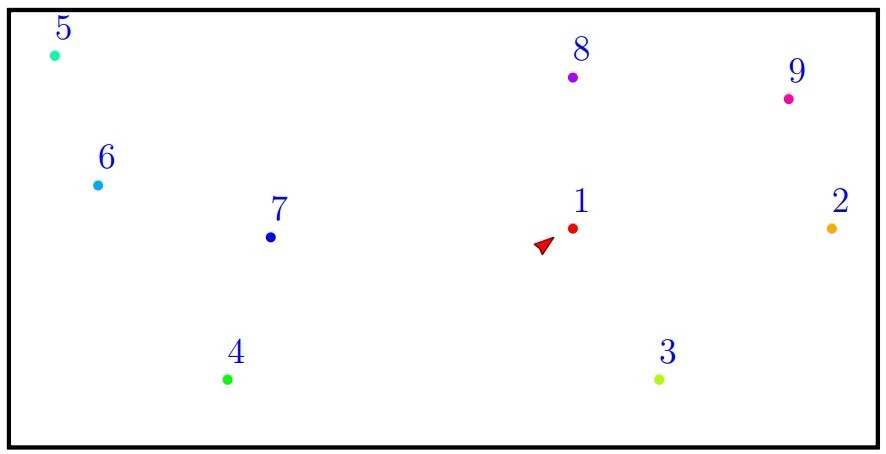
\includegraphics[scale=0.2]{figs/obs.jpg}  \\ 
%         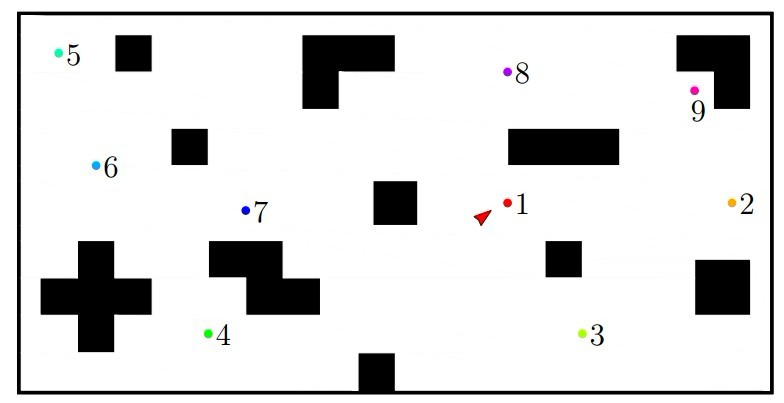
\includegraphics[scale=0.23]{figs/clutter.jpg}  
%       \end{figure}
%     \end{column}
%     \begin{column}[b]{0.45\textwidth}
%     \begin{figure}
%       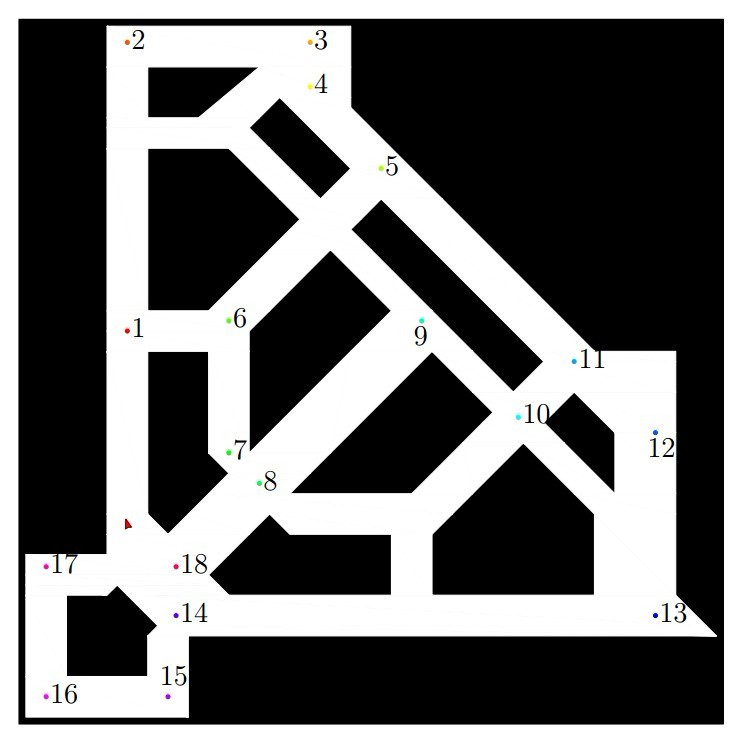
\includegraphics[scale=0.25]{figs/office.jpg}    
%     \end{figure}
%   \end{column}
% \end{columns}
% \end{frame}

\begin{frame}{Comparison of Efficiency and Accuracy}
\begin{table}
  \scriptsize\centering
    \begin{tabular}{ccccccc} 
    \hline
    Range & \multicolumn{2}{c}{Obstacle-free} & \multicolumn{2}{c}{Clutter} & \multicolumn{2}{c}{Office-like}\\
    Space & Time(s) &Approx.Ratio& Time(s) &Approx.Ratio& Time(s) &Approx.Ratio \\
    \hline
    $\mathcal{R}_{disk}$ & 0.163 & 0.155 & 0.162 & 0.155  & 0.292 & 0.220 \\ 
    \hline
    $\mathcal{R}_{rect}$ & 0.396 & 0.642  & 0.441 & 0.632 & 0.415 & 0.661 \\
    \hline
    $\mathcal{R}_{dblrect}$ & 1.021 & 0.684 & 1.122 & 0.691 & 1.491 & 0.720 \\
    \hline
    $\mathcal{I}$ & 10.074 & 1.000 & 10.218 & 1.000 & 26.895 & 1.000 \\
    \hline
    \end{tabular}
    \caption{Experimental results: computation time and approximation
      ratio for range spaces and I-space in three test environments.}
    \label{tab:exp-data}
\end{table}
\end{frame}
% \begin{frame}{Comparison of Success Rate}{Office-like Environment}
%   \begin{figure}
%     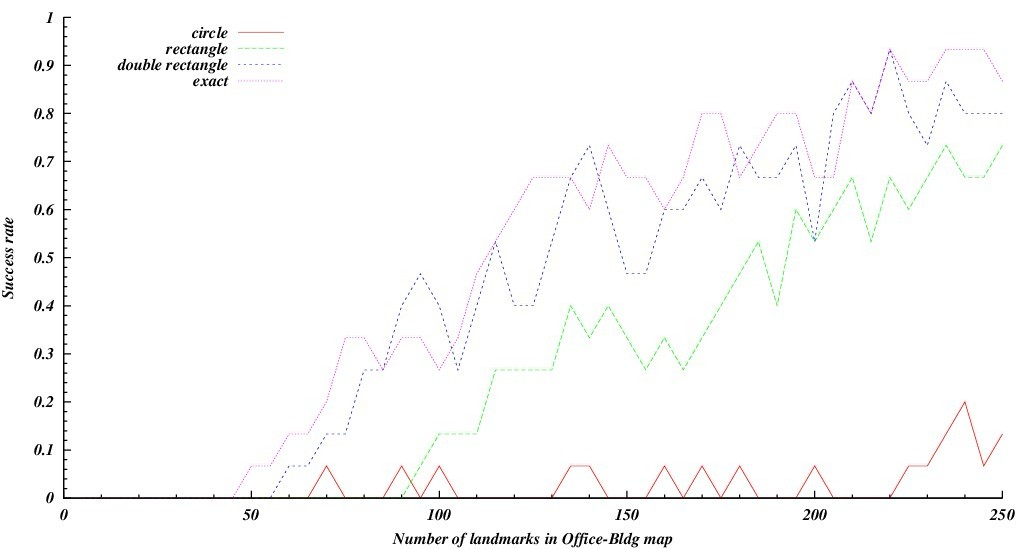
\includegraphics[width=6cm]{figs/rate-office.jpg}
%     \caption{For an environment with complex obstacles, $\mathcal{R}_{dblrest}$ shows
%       better performance than using $\mathcal{R}_{disk}$ or $\mathcal{R}_{rect}$ and
%       achieve almost same success rate compared to the true I-states.}
%   \end{figure}
% \end{frame}

% \begin{frame}{Computation and Approximation ratio}{Obstacle-clutter Environment}
% \begin{figure}
%     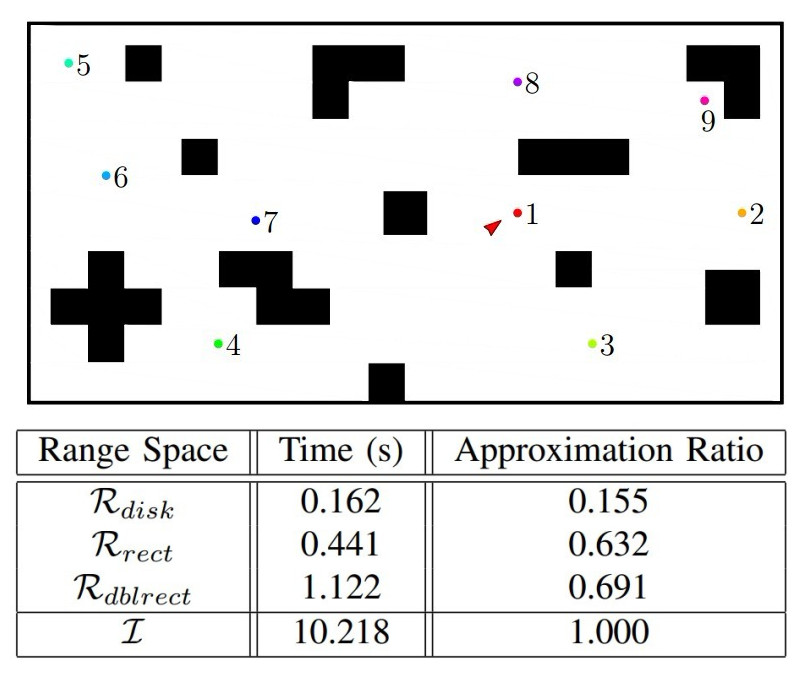
\includegraphics[width=6cm]{figs/clutter_tab.jpg}
%     \caption{For an environment with complex obstacles, $\mathcal{R}_{dblrest}$ shows
%       better performance than using $\mathcal{R}_{disk}$ or $\mathcal{R}_{rect}$ and
%       achieve almost same success rate compared to the true I-states.}
% \end{figure}
% \end{frame}

% \begin{frame} \frametitle{Comparison of Success Rate}{Obstacle-clutter Environment}
% \begin{figure}
%     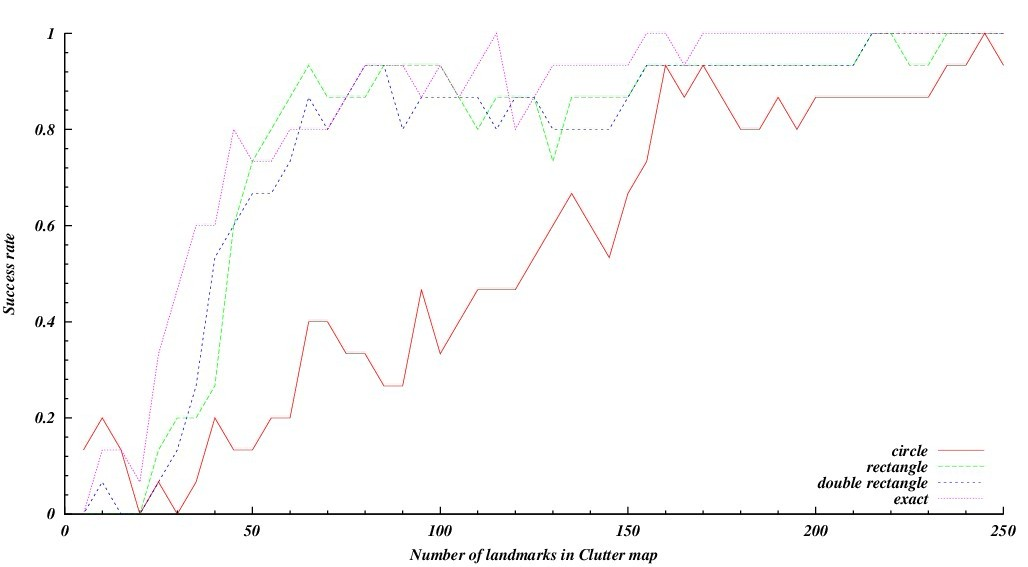
\includegraphics[width=6cm]{figs/rate-clutter.jpg}
%     \caption{Using $\mathcal{R}_{rect}$, $\mathcal{R}_{dblrest}$, achieve similar
%       performance to the true	I-state. Using $\mathcal{R}_{disk}$ yields lower success
%       rate due to the high possibility of collisions.}
% \end{figure}
% \end{frame}
%\section[Conclusions]{Conclusions}
\begin{frame}{Conclusions}
  \begin{itemize}
  \item CGA is effective for representing a robot's uncertain information about
    the current state.
  \item The form of double-rectangle is more accurate in approximating the non-convex
    \emph{I-state}.
  \item The robot can complete the navigation task using approximated I-state with
    low approximation accuracy.
  \end{itemize}
\end{frame}

\section{Multi-Robot Formation}
\begin{frame}{Related Work}{Formation using virtual force}
   \begin{columns}[T] 
    \begin{column}{.45\textwidth}
      \scriptsize{W. Spears, D. Spears, J. Hamann and R. Heil, 2004}
      \begin{figure}
        \centering
        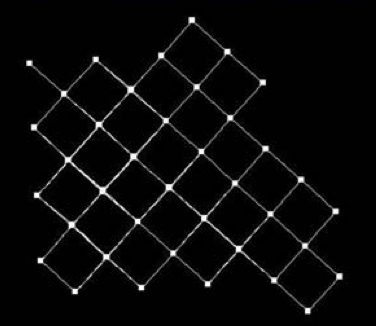
\includegraphics[height=1in]{figs/spears1.png}
      \end{figure}
    \end{column}%
    \begin{column}{.45\textwidth}
      \scriptsize{I. Navarro, J. Pugh, A. Martinoli, and
        F. Matia, 2008}
      \begin{figure}
        \centering
        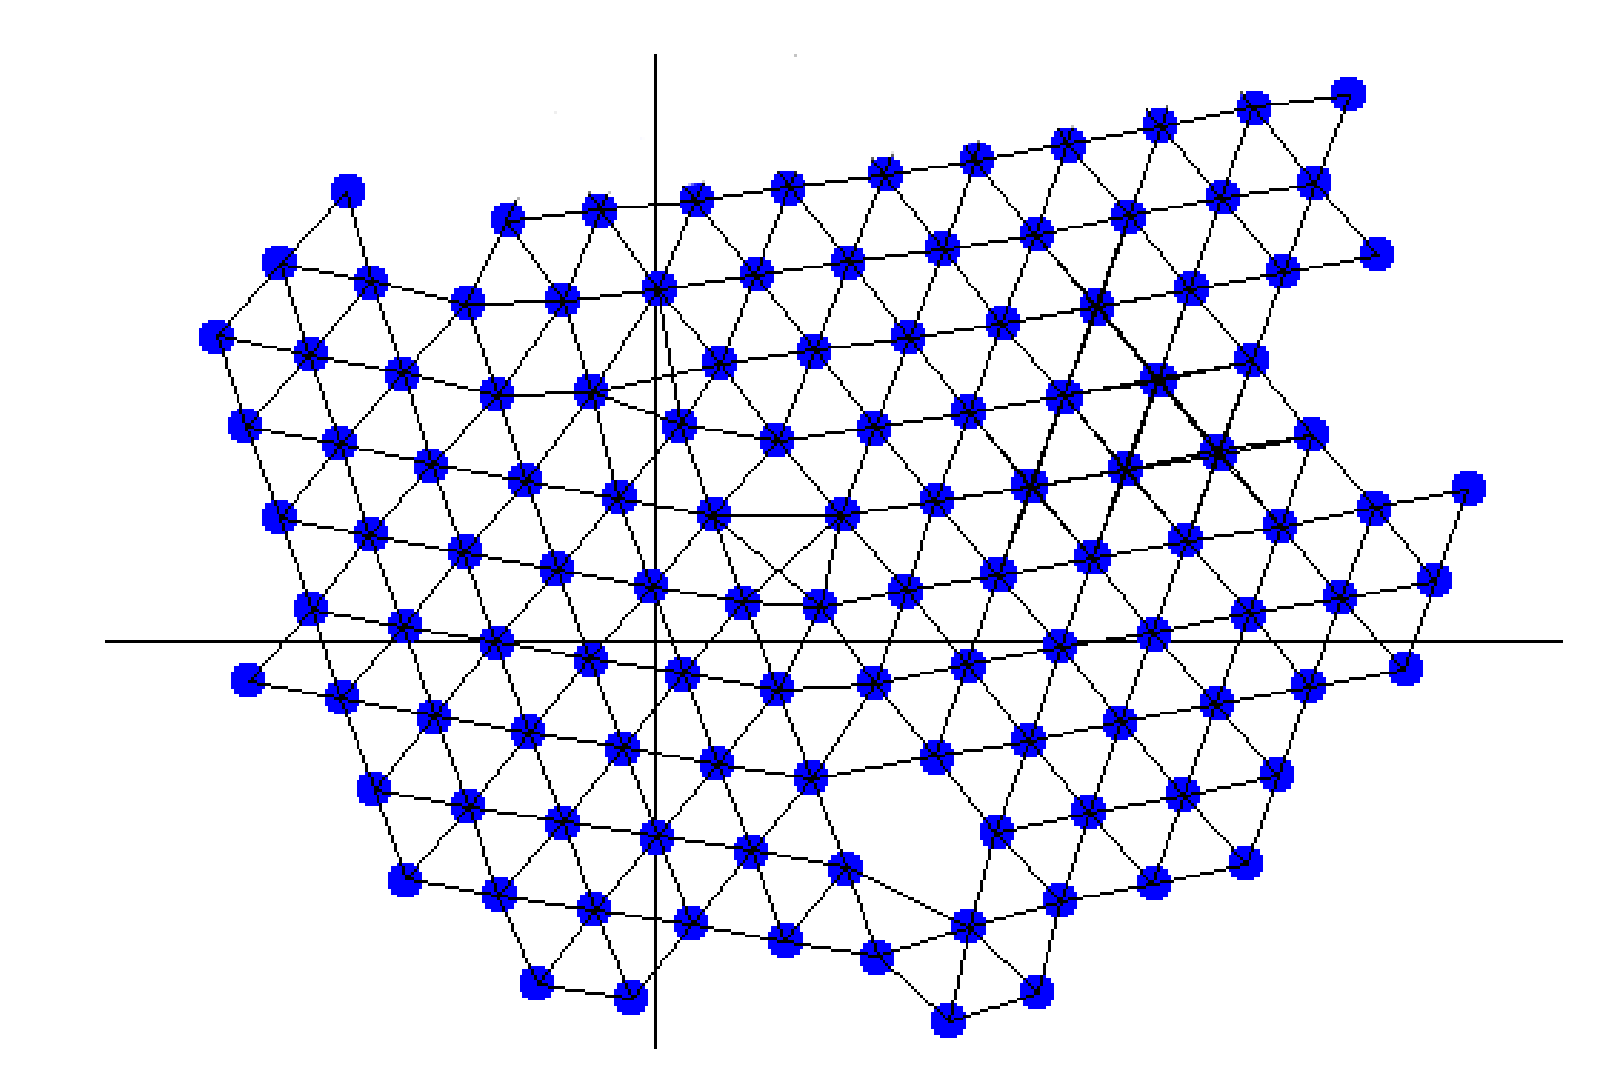
\includegraphics[height=1in]{figs/navarro.png}
      \end{figure}      
    \end{column}
  \end{columns}
  \vspace{3mm}
  \begin{columns}[T] 
    \begin{column}{.45\textwidth}
      \begin{figure}
        \centering
        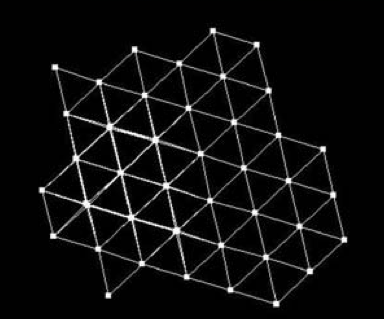
\includegraphics[height=1in]{figs/spears2.png}     
      \end{figure}  
    \end{column}%
    \begin{column}{.45\textwidth}
      \scriptsize{S. Prabhu, W. Li, J. McLurkin, 2012}
      \begin{figure}
        \centering
        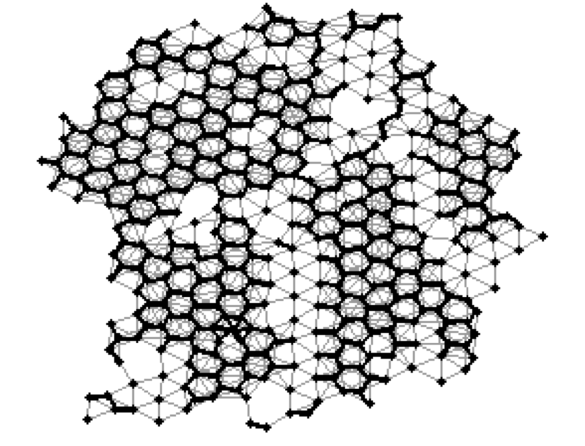
\includegraphics[height=1in]{figs/james.png}
      \end{figure}
    \end{column}
  \end{columns}
\end{frame}

\begin{frame}{Motivation}{}
  \begin{block}{Question: How to use one algorithm to generate
      various (repeating) lattice pattern formations?}
    \begin{columns}
    \begin{column}{.45\textwidth}
      \begin{figure}
        \centering
        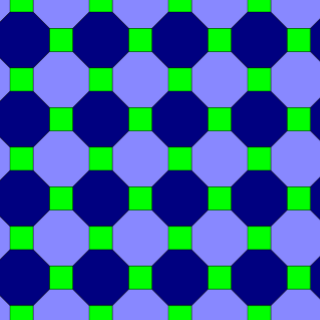
\includegraphics[height=1.5in]{figs/tessellation2.png}
      \end{figure}
    \end{column}
    \begin{column}{.45\textwidth}
       \begin{figure}
         \centering
        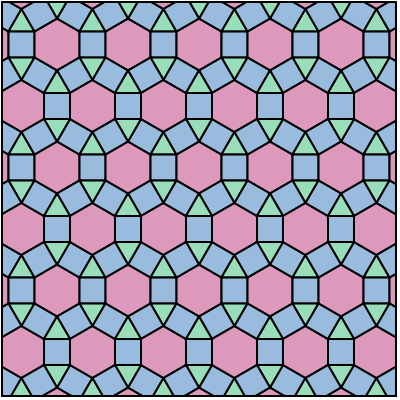
\includegraphics[height=1.5in]{figs/tessellation1.png}
      \end{figure}
    \end{column}
  \end{columns} 
  \end{block}
\end{frame}
\begin{frame}{Simulation Example}{Square formation with 10 robots}
  \begin{center}
  \includemovie[toolbar, poster, autoplay]{5cm}{5cm}{videos/square10.mp4}
  \end{center}
\end{frame}
%%%%%%%%%%%%%%%%
\begin{frame}{Robot Model}{}
%\begin{block}{}
  \begin{columns}[T] % align columns
      \begin{column}{.55\textwidth}
        \begin{itemize}
        \item Differential Drive robots.
        \item Each robot has an unique \textbf{ID}.
        \item Use a vector $p = [x, y,
          \theta]^T$ to represent robot's \textbf{pose}.
        \item Each robot has a \textbf{range} within which it can
          sense and communicate with other robots.
        \item Each robot gets \textbf{observation} of its neighbors'
          IDs and relative poses in its body frame.
        \end{itemize}
      \end{column}%
      % right column
      \begin{column}{.45\textwidth}
        \begin{figure}
          \centering
          \begin{tikzpicture}[scale=0.55]
            \draw[dotted, violet, fill=violet!10] (3, 3) circle (3.2);
            \draw[fill=red] (3,3) -- (2.75,3) -- (3.25,3.25) -- (3,2.75)   	-- cycle;
            \node[color=red] at (3, 2.3) {$r_i$};           
            \draw[fill=blue!50] (0.5,4.5) -- (0.33,4) -- (0.5,4.125) -- (0.67,4) 	-- cycle;
            \draw[fill=blue!50] (4,5) -- (3.75,5.5) -- (3.75,5.25) -- (3.5,5.25)   	-- cycle;
            \draw[fill=blue!50] (1,1.5) -- (1.25,1) -- (1.25,1.25) -- (1.5,1.25)   	-- cycle;
            \draw[fill=blue!50] (5,2.92) -- (4.5,2.75) -- (5,2.58) -- (4.875,2.75)  -- cycle;
            \draw[fill=green!50] (-0.5,0.5) -- (-0.5,0.75) -- (-0.75,0.25) -- (-0.25,0.5)  -- cycle;
          \end{tikzpicture}
        \end{figure}
        \begin{center}
          Robot $r_i$ has 4 neighbors
        \end{center}
      \end{column}%
    \end{columns}
\end{frame}
%%%%%%%%%%%%%%%%

\section{Lattice Graph}
% definition of lattice graph
\begin{frame}{Input: Lattice Graph}
    %\begin{bclogo}[logo=\bccrayon, couleur=orange!10, arrondi=0.2, ombre=true]{Definition}
  \begin{definition}
    A \textbf{lattice graph} is a strongly connected directed
      multigraph in which each edge $e$ is labeled with a rigid body
      transformation $T(e)$ and each $\edge{v}{T(e)}{w}$ has an
      inverse edge $\edge{w}{T(e)^{-1}}{v}$.  
    %\end{bclogo}
    \end{definition}
    \begin{columns}[T] % align columns
      \begin{column}{.45\textwidth}
        \begin{figure}
          \centering
          \begin{tikzpicture}[->,>=stealth',shorten >=5pt,auto,node distance=1cm]
            \tikzstyle{every state}=[fill=purple,draw=none, text=white]
            \node[state, scale=0.6] (A)         {$0$};
            \path (A) edge [loop above] node {\footnotesize{Tr(0, 40)}} (A)
                      edge [loop left]  node {\footnotesize{Tr(-40,0)}} (A)
                      edge [loop below] node {\footnotesize{Tr(0, -40)}} (A)
                      edge [loop right] node {\footnotesize{Tr(40, 0)}} (A);
          \end{tikzpicture}
        \end{figure}
      \end{column}%
      \begin{column}{.45\textwidth}
        \begin{figure}
          \centering
          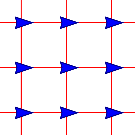
\includegraphics[scale=1]{figs/squarelattice}
        \end{figure}
      \end{column}%
    \end{columns}
\end{frame}

\begin{frame}{Role Function}
  %\begin{block}{}
  %\begin{bclogo}[logo=\bccrayon, couleur=orange!10, arrondi=0.1,
  %ombre=true]{Definition}
  \begin{definition}
    \small{Given a lattice graph $G=(V, E)$ and a set of robots $R = \{
    r_1, \ldots, r_n \}$, $R$ \textbf{satisfies} $G$ if
    there exists a role function $f: R \rightarrow V$ that preserves
    the neighborhood structure of $G$.
    \\
    Specifically, for any $i$ and $j$, if $r_i$ and $r_j$ are neighbors, 
    there must exist an edge
    $e_{ij}: \edge{f(r_i)}{}{f(r_j)}$ in $E$, such that
    $ T(r_j) = T(r_i) T(e_{ij})$.}
  %\end{bclogo}
  \end{definition}
%\hrule 
  \begin{columns}[T] 
    \begin{column}{.4\textwidth}
      \begin{figure}
        \centering
        % 
\includegraphics[scale=0.38]{figs/hex}
        \begin{tikzpicture}[->,>=stealth',shorten >=5pt,auto,node
          distance=1cm]
            \tikzstyle{every state}=[fill=purple, draw=none, text=white]
            \node[state, scale=0.6] (A) at (0,0)    {$0$};
            \node[state, scale=0.6, fill=cyan] (B) at (3,0)  {$1$};
            \path (A) edge [bend left=10] node {\scriptsize{Tr(0, 40)}} (B)
                  (A) edge [bend left=45] node {\scriptsize{Tr(-35,-20)}} (B)
                  (A) edge [bend left=90] node
                  {\scriptsize{Tr(35,-20)}} (B)
                  (B) edge [bend left=10]  node {\scriptsize{Tr(-40,0)}} (A)
                  (B) edge [bend left=45]  node
                  {\scriptsize{Tr(35,20)}} (A)
                  (B) edge [bend left=90]  node {\scriptsize{Tr(-35,20)}} (A);
        \end{tikzpicture}
      \end{figure}
    \end{column}%
    \begin{column}{.5\textwidth}
      \begin{figure}
        \centering
        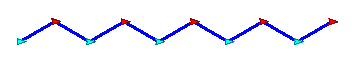
\includegraphics[width=0.75\linewidth]{figs/bad-hexagon}
      \end{figure}
      \begin{figure}
        \centering
        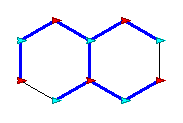
\includegraphics[scale=0.8]{figs/good-hexagon}
        \end{figure}
    \end{column}%
  \end{columns}
  %\end{block}
\end{frame}


\subsection{Algorithm}
\begin{frame}{Algorithm}
  \begin{block}{General Description}
  \begin{columns}[T] % align columns
   \begin{column}{.45\textwidth}
     Robot broadcasts message containing its
     \begin{itemize}
     \item \textcolor{red}{authority} 
     \item \textcolor{red}{matching}.
     \end{itemize}

      \begin{enumerate}
      \item Form tree structure.
      \item Use tree structure to computer local task assignment.
      \item Make movement decision.
      \end{enumerate}
    \end{column}%
    \begin{column}{.45\textwidth}
      \begin{animateinline}[
        begin={%
          \begin{tikzpicture}%
           [post/.style={->,>=stealth', semithick, draw=blue!50},
            node/.style={circle,fill=red!20,draw,font=\sffamily\small}]%
            \useasboundingbox (0,0) rectangle (5,5);
          },
          end={\end{tikzpicture}}
        ]{10}
         %\draw[dotted, violet, fill=violet!10] (3, 3) circle (3.5);
         \draw[fill=blue!50] (3,3) -- (2.75,3) -- (3.25,3.25) -- (3,2.75)  -- cycle;
         % \node[color=black] at (3, 4.5) {broadcast Message};           
         \draw[fill=blue!50] (0.5,4.5) -- (0.33,4) -- (0.5,4.125) -- (0.67,4) -- cycle;
         \draw[fill=blue!50] (1,1.5) -- (1.25,1) -- (1.25,1.25) --
         (1.5,1.25) -- cycle;
         \newframe*
         \multiframe{10}{rP = 0.1 +.1, r = 1 + 1}{ 
           \draw[fill=blue!50] (3,3) -- (2.75,3) -- (3.25,3.25) -- (3,2.75)  -- cycle;
           \node[color=black] at (3, 4.5) {broadcast Message};           
           \draw[fill=blue!50] (0.5,4.5) -- (0.33,4) -- (0.5,4.125) -- (0.67,4) -- cycle;
           \draw[fill=blue!50] (1,1.5) -- (1.25,1) -- (1.25,1.25) --
           (1.5,1.25) -- cycle;
           \path (3,3) -- (1.25, 1.25) node[pos=\rP] (q){};
           \draw[post] (3,3) -- (q.west);
           
           \path (3,3) -- (0.5, 4.125) node[pos=\rP] (q){};
           \draw[post] (3,3) -- (q.west);
           
           \path (1.5, 1.25) -- (3,2.5) node[pos=\rP] (q){};
           \draw[post] (1.5, 1.25) -- (q.west);
           
           \path (1.25, 1.5) -- (0.5, 4.125) node[pos=\rP] (q){};
           \draw[post] (1.25, 1.5) -- (q.south);
           
           \path (0.5, 4.5) -- (3.25, 3.25) node[pos=\rP] (q){};
           \draw[post] (0.5, 4.5) -- (q.north);

           \path (0.33, 4) -- (1, 1.5) node[pos=\rP] (q){};
           \draw[post] (0.33, 4) -- (q.north);
        }
        \newframe*
        \multiframe{10}{rP = 0.1 +.1, r = 1 + 1}{ 
         \draw[fill=red] (3,3) -- (2.75,3) -- (3.25,3.25) -- (3,2.75)  -- cycle;
         \node[color=red] at (3, 2.3) {$root$};           
         \draw[fill=blue] (0.5,4.5) -- (0.33,4) -- (0.5,4.125) --
         (0.67,4) 	-- cycle;
         \node[color=blue] at (1, 3.75) {$descendant$};           
         \draw[fill=blue] (1,1.5) -- (1.25,1) -- (1.25,1.25) -- (1.5,1.25)  -- cycle;
         \node[color=blue] at (2.5,1.5) {$descendant$};
         \node[color=black] at (3, 4.5) {Form Tree Structure};
         \path (3,3) -- (1.25, 1.25) node[pos=\rP] (q){};
         \draw[post, color=red] (3,3) -- (q);
           
         \path (3,3) -- (0.5, 4.125) node[pos=\rP] (q){};
         \draw[post, color=red] (3,3) -- (q);
        }
        \newframe*
        \multiframe{10}{r = 1 + 1}{ 
          \draw[fill=red] (3,3) -- (2.75,3) -- (3.25,3.25) -- (3,2.75)  -- cycle;
          \draw[fill=blue] (0.5,4.5) -- (0.33,4) -- (0.5,4.125) --
         (0.67,4) 	-- cycle;
         \draw[fill=blue] (1,1.5) -- (1.25,1) -- (1.25,1.25) -- (1.5,1.25)  -- cycle;
         \node[color=black] at (3, 4.5) {Assign Task};  
         %\path (3,3) -- (1.25, 1.25) node[pos=\rP] (q){};
         \draw[post, color=red] (3,3) -- (1.25, 1.25);
         % \path (3,3) -- (0.5, 4.125) node[pos=\rP] (q){};
         \draw[post, color=red] (3,3) -- (0.5,4.125);
         \draw[red, dotted] (1,3) -- (0.75,3) -- (1.25,3.25) -- (1,2.75) -- cycle;
         \draw[red, dotted] (3,1) -- (2.75,1) -- (3.25,1.25) -- (3,0.75) -- cycle;
         \draw[dashed](1.25,1.25) -- (3,1);
         \draw[dashed](0.5,4.125) -- (1,3);
        }
        \newframe*
        \multiframe{10}{r = 1 + 1}{ 
          \draw[fill=red] (3,3) -- (2.75,3) -- (3.25,3.25) -- (3,2.75)  -- cycle;
          \node[color=black] at (3, 4.5) {Movement Control};  
          \draw[post, color=red] (3,3) -- (1,3);
          \draw[post, color=red] (3,3) -- (3,1);
          \draw[fill=blue] (1,3) -- (0.75,3) -- (1.25,3.25) -- (1,2.75) -- cycle;
          \draw[fill=blue] (3,1) -- (2.75,1) -- (3.25,1.25) -- (3,0.75) -- cycle;
        }
      \end{animateinline}
    \end{column}%
  \end{columns}
\end{block}
\end{frame}
%%%%%%%%%%%%%%%%
\subsection{Robot Authority}
\begin{frame}{Authority}
  \begin{block}{Define authority and comparison operator}
    %\begin{bclogo}[logo=\bccrayon,couleur=orange!10, arrondi=0.1,ombre=true]{}
      \begin{definition}
      \small{An \textbf{authority} is an ordered list of robot IDs
        $$(\id_1, \ldots, \id_k)$$
        The first ID in the list, $\id_1$ is called the \textbf{root} ID.
        The final ID in the list, $\id_k$ is called the \textbf{sender} ID.}
%        The number of IDs in the list is called its \textbf{length}}
    %\end{bclogo}
    \end{definition}
    \begin{definition}
    %\begin{bclogo}[logo=\bccrayon,couleur=orange!10, arrondi=0.1, ombre=true]{}
      \small{Authority $A_2$ is \textbf{higher than} $A_1$ if:}
      \begin{itemize}
      \item \small{root ID of $A_2 >$ root ID of $A_1$, or}
      \item \small{length of $A_2 <$  length of $A_1$ if they have the same root, or}
      \item \small{sender ID of $A_2 >$ sender ID of $A_1$ if they have the same root and length.}
      \end{itemize}
    %\end{bclogo}
    \end{definition}
  \end{block}
\end{frame}

%%%%%%%%%%%%%%%%

% help me iron out the bugs or give me some comment and suggestions
\begin{frame}{1.Construct Authority Tree}{Decide to be root or descendant}
  \begin{block}{The robots use these authorities to establish a
      collection of authority trees}
    \begin{enumerate}
    \item Discards any message in which the authority contains its
      own ID.
    \item Forms an authority containing only its own ID,
      compares it with the authorities of remaining messages and
      selects the highest authority.
    \end{enumerate} 
  \begin{columns}[T] % align columns
    \begin{column}{.45\textwidth}
      \begin{itemize}
      \item If its authority is the highest, then it is
        a \textcolor{red}{root};
      \item Otherwise, it selects the one who sends the highest
        authority as its parent. Append its own ID to the highest
        authority to create its own authority. 
      \end{itemize}     
    \end{column}%
    \begin{column}{.45\textwidth}
       \begin{animateinline}[
        begin={%
          \begin{tikzpicture}%
           [post/.style={->,>=stealth', thick, draw=blue!50},
            node/.style={circle,fill=red!20,draw,font=\sffamily\small}]%
            \useasboundingbox (0,1) rectangle (5,5);
          },
          end={\end{tikzpicture}}
        ]{10}
        \draw[dashed, blue] (3, 4) circle (3);
        % center is (3,4)
        \draw[fill=blue!50] (3,4) -- (2.75,4) -- (3.25,4.25) -- (3,3.75)  -- cycle;
        \node[color=blue] at (2.75, 3.5) {$(2)$};
        % center is (0.5, 4.5)
        \draw[dashed, green] (0.5,4.5) circle (2.8);
        \draw[fill=green!50] (0.5,4.5) -- (0.33,4) -- (0.5,4.125) --
        (0.67,4) -- cycle;
        \node[color=green] at (0.5, 3.75) {$(4)$};
        % center is (3.75,2)
        \draw[dashed, red] (3.75,2) circle (2.5);
         \draw[fill=red!50] (3.5,2.5) -- (3.75,2) -- (3.75,2.25) --
         (4,2.25) -- cycle;
         \node[color=red] at (3.3, 2) {$(3)$};
         %%%%
        \newframe*
        \multiframe{10}{rP= 0.1+ .1, r = 1 + 1}{ 
          \draw[dashed, blue] (3, 4) circle (3);
          % center is (3,4)
          \draw[fill=blue!50] (3,4) -- (2.75,4) -- (3.25,4.25) --
          (3,3.75)  -- cycle;
          \node[color=blue] at (2.75, 3.5) {$(4,2)$};
          % center is (0.5, 4.5)
          \draw[dashed, green] (0.5,4.5) circle (2.8);
          \draw[fill=green!50] (0.5,4.5) -- (0.33,4) -- (0.5,4.125) --
          (0.67,4) -- cycle;
          \node[color=green] at (0.5, 3.75) {$(4)$};
          % center is (3.75,2)
          \draw[dashed, red] (3.75,2) circle (2.5);
          \draw[fill=red!50] (3.5,2.5) -- (3.75,2) -- (3.75,2.25) --
          (4,2.25) -- cycle;
          \node[color=red] at (3.3, 2) {$(3)$};
          \path (0.5,4.125) -- (3,4) node[pos=\rP] (q){};
          \draw[post] (0.5,4.125) -- (q);
        }
        \newframe*
        \multiframe{10}{r = 1 + 1}{ 
          \draw[dashed, blue] (3, 4) circle (3);
          % center is (3,4)
          \draw[fill=blue!50] (3,4) -- (2.75,4) -- (3.25,4.25) --
          (3,3.75)  -- cycle;
          \node[color=blue] at (2.75, 3.5) {$(4,2)$};
          % center is (0.5, 4.5)
          \draw[dashed, green] (0.5,4.5) circle (2.8);
          \draw[fill=green!50] (0.5,4.5) -- (0.33,4) -- (0.5,4.125) --
          (0.67,4) -- cycle;
          \node[color=green] at (0.5, 3.75) {$(4)$};
          % center is (3.75,2)
          \draw[dashed, red] (3.75,2) circle (2.5);
          \draw[fill=red!50] (3.5,2.5) -- (3.75,2) -- (3.75,2.25) --
          (4,2.25) -- cycle;
          \node[color=red] at (3, 2) {$(4,2,3)$};
          \draw[post] (0.5,4.125) -- (2.87,4);
        }
         \newframe*
         \multiframe{10}{rP = 0.1 +.1, r = 1 + 1}{ 
           \draw[dashed, blue] (3, 4) circle (3);
          % center is (3,4)
          \draw[fill=blue!50] (3,4) -- (2.75,4) -- (3.25,4.25) --
          (3,3.75)  -- cycle;
          \node[color=blue] at (2.75, 3.5) {$(4,2)$};
          % center is (0.5, 4.5)
          \draw[dashed, green] (0.5,4.5) circle (2.8);
          \draw[fill=green!50] (0.5,4.5) -- (0.33,4) -- (0.5,4.125) --
          (0.67,4) -- cycle;
          \node[color=green] at (0.5, 3.75) {$(4)$};
          % center is (3.75,2.25)
          \draw[dashed, red] (3.75,2) circle (2.5);
          \draw[fill=red!50] (3.5,2.5) -- (3.75,2) -- (3.75,2.25) --
          (4,2.25) -- cycle;
          \node[color=red] at (3, 2) {$(4,2,3)$};
          \draw[post] (0.5,4.125) -- (2.87,4);

          \path (3,4) -- (3.75, 2.25) node[pos=\rP] (q){};
          \draw[post] (3,4) -- (q);        
        }
      \end{animateinline}
    \end{column}
  \end{columns}
\end{block}
\end{frame}
%%%%%%%%%%%%%%%%

\begin{frame}{Matching}{}
 \begin{block}{}
  % Given a robot $r_i$ and a role vertex $v_i$ for that
  % robot, let the lattice graph edge set $L=\{\emptyset,e_{ij}, e_{ik},
  % \ldots\}$ be the set that contains a null value $\emptyset$ and all
  % outgoing edges from vertex $v_i$. Let $Q=\{\id(r_a), \id(r_b),
  % \ldots \}$ be the set that contains the IDs of the neighbors of $r_i$.  
  %\begin{columns}[T] 
    %\begin{column}{.45\textwidth}
   %\begin{bclogo}[logo=\bccrayon,arrondi=0.1]{} 
   \begin{definition}    
     A \textbf{matching} for a robot is a function $\eta : \{\id(r_a),
     \id(r_b), \ldots \} \rightarrow \{\emptyset,e_{ij}, e_{ik},
     \ldots\} $ that associates each neighbor ID with either a lattice
     graph edge from its role vertex or with the null value
     $\emptyset$.
   \end{definition}
   %\end{bclogo}   
   % \end{column}%
   % \begin{column}{.45\textwidth}
      \begin{figure}
        % \centering
        \begin{tikzpicture}[
          fsnode/.style={},
          ssnode/.style={},
          every fit/.style={ellipse,draw,inner sep=0pt,text width=1cm},
          ->,shorten >= 2pt,shorten <= 2pt
          ]
          % the vertices of Q
          \begin{scope}[start chain=going below,node distance=1mm]
            \foreach \i/\xcoord in {1/\id(r_a),2/\id(r_b),3/\vdots, 4/\id(r_c)}
            \node[fsnode,on chain] (f\i) {$\xcoord$};
          \end{scope}
          % the vertices of L
          \begin{scope}[xshift=3cm,start chain=going below,node distance=1mm]
            \foreach \i/\xcoord in {5/e_{ij},6/e_{ik}, 7/\vdots, 8/\emptyset}
            \node[ssnode,on chain] (s\i) {$\xcoord$};
          \end{scope}         
          % the set U
          %\node [myblue,fit=(f1) (f4),label=below:$Q$] {};
          \node [myblue,fit=(f1) (f4), label=above:$$] {};
          % the set V
          \node [mygreen,fit=(s5) (s8), label=above:$$] {};
          % the edges
          \draw (f1) -- (s6);
          \draw (f2) -- (s5);
          \draw (f4) -- (s8);
        \end{tikzpicture}
      \end{figure}
    %\end{column}%
  %\end{columns}
  \end{block}
\end{frame}
%%%%%%%%%%%%%%%%

% installation on Microsoft Windows Cont'd
\begin{frame}{2. Local Task Assignment}{Hungarain Algorithm}
  To compute an optimal matching of a robot with $N$ neighbors and $E$
  out-going edges of its role in the lattice graph, define a weight
  matrix of size $N \times \max(N, E)$ and apply
  \textcolor{scred}{Hungarian Algorithm} (Harold W. Kuhn, 1955).
    \begin{columns}[T] % align columns
      \begin{column}{.5\textwidth}
        \begin{enumerate}
        \item Each row corresponds to a neighbor;
        \item Each column corresponds to an out-going edge of robot's
          role or a null value $\emptyset$.
        \item The entries of the matrix are the Euclidean distance
          between current position of each neighbor and the desired
          position if matched with a lattice graph edge.
        \end{enumerate}
      \end{column}%
      \begin{column}{.4\textwidth}
        \vspace{3mm}
           \begin{animateinline}[
             begin={%
               \begin{tikzpicture}%
                 [post/.style={->,>=stealth', thin, draw=blue!50},
                 node/.style={circle,fill=red!20,draw,font=\sffamily\small},
                 scale=0.8]%
                 %\useasboundingbox (0,0) rectangle (5,5);
               },
               end={\end{tikzpicture}}
             ]{10}
             \draw[fill=red] (3,3) -- (2.75,3) -- (3.25,3.25) -- (3,2.75) -- cycle;
             \draw[fill=blue!50] (0.5,4.5) -- (0.33,4) -- (0.5,4.125)
             -- (0.67,4) -- cycle;
             \draw[fill=blue!50] (4,5) -- (3.75,5.5) -- (3.75,5.25) -- (3.5,5.25)   	-- cycle;
             \draw[fill=blue!50] (1,2.5) -- (1.25,2) -- (1.25,2.25) -- (1.5,2.25)   	-- cycle;
             \draw[fill=blue!50] (5,2.92) -- (4.5,2.75) -- (5,2.58) -- (4.875,2.75)  -- cycle;
             \draw[fill=blue!50] (-0.5,2.5) -- (-0.5,2.75) -- (-0.75,2.25) -- (-0.25,2.5)  -- cycle;
             \draw[color=red] (4,4) -- (3.75,4) -- (4.25,4.25) -- (4,3.75) -- cycle;
             \draw[color=red] (2,2) -- (1.75,2) -- (2.25,2.25) -- (2,1.75) -- cycle;
             \draw[color=red] (2,4) -- (1.75,4) -- (2.25,4.25) -- (2,3.75) -- cycle;
             \draw[color=red] (4,2) -- (3.75,2) -- (4.25,2.25) -- (4,1.75) -- cycle;
             \newframe*
             \multiframe{10}{r = 1 + 1}{ 
               \draw[fill=red] (3,3) -- (2.75,3) -- (3.25,3.25) -- (3,2.75)   	-- cycle;
               \draw[fill=blue!50] (0.5,4.5) -- (0.33,4) -- (0.5,4.125) -- (0.67,4) 	-- cycle;
               \draw[fill=blue!50] (4,5) -- (3.75,5.5) -- (3.75,5.25) -- (3.5,5.25)   	-- cycle;
               \draw[fill=blue!50] (1,2.5) -- (1.25,2) -- (1.25,2.25) -- (1.5,2.25)   	-- cycle;
               \draw[fill=blue!50] (5,2.92) -- (4.5,2.75) -- (5,2.58) -- (4.875,2.75)  -- cycle;
               \draw[fill=blue!50] (-0.5,2.5) -- (-0.5,2.75) -- (-0.75,2.25) -- (-0.25,2.5)  -- cycle;
               
               \draw[color=red] (4,4) -- (3.75,4) -- (4.25,4.25) -- (4,3.75) -- cycle;
               \draw[color=red] (2,2) -- (1.75,2) -- (2.25,2.25) -- (2,1.75) -- cycle;
               \draw[color=red] (2,4) -- (1.75,4) -- (2.25,4.25) -- (2,3.75) -- cycle;
               \draw[color=red] (4,2) -- (3.75,2) -- (4.25,2.25) -- (4,1.75) -- cycle;
               
               \draw[dashed](0.5, 4.25) -- (2,4);
               \draw[dashed](1.25,2.25) -- (2,2);
               \draw[dashed](3.75,5.25) -- (4,4);
               \draw[dashed](4.75,2.75) -- (4,2);
             }
        \end{animateinline}
        \vspace{3mm}
        \begin{flushleft}
          \footnotesize{5 neighbors, 4 out-going edges.}
        \end{flushleft}
        
      \end{column}%
    \end{columns}
\end{frame}
%%%%%%%%%%%%%%%%

\begin{frame}{3. Robot Movement Strategy}{}
  % Define block styles
\tikzstyle{decision} = [diamond, draw, fill=red!10, 
    text width=4em, text badly centered, node distance=3cm, inner sep=0pt]
\tikzstyle{block} = [rectangle, draw, fill=blue!10, 
    text width=5em, text centered, rounded corners]%, minimum height=2em]
\tikzstyle{line} = [draw, -latex']

\begin{figure}    
\centering
\begin{tikzpicture}
    % Place nodes
    \node [block] (init) {\footnotesize{Start}};
    \node [decision, below of=init, node distance=2cm] (decide) {\footnotesize{Root?}};
    % \node [block, below of=decide, node distance=2cm] (root) {\footnotesize{root}};
    \node [block, below of=decide, node distance=2cm] (stop) {\footnotesize{Stay}};
    % \node [block, right of=decide, node distance=3cm] (descendant) {\footnotesize{Descendant}};
    \node [decision, right of=decide, node distance=3.5cm] (decideagain) {\footnotesize{Assigned?}};
    \node [block, right of=decideagain, node distance=3.5cm, text width=6em] (away)
    {\footnotesize{Move away from parent}};
    \node [block, below of=decideagain, node distance=3cm, text width=9em] (go)
    {\footnotesize{Move towards assigned destination}};
    % Draw edges
    \path [line] (init) -- (decide);
    \path [line] (decide) -- node [xshift=-0.5cm]{yes}(stop);
    \path [line] (decide) -- (stop);
    \path [line] (decide) -- node [yshift=0.3cm] {no} (decideagain);
    \path [line] (decideagain) -- node [yshift=0.3cm] {no} (away);
    \path [line] (decideagain) -- node [xshift=-0.5cm] {yes} (go);
  \end{tikzpicture}
  \end{figure}
\end{frame}

% \begin{frame}{Simulation}{Line formation with 6 robots}
%   \begin{center}
%   \includemovie[toolbar,poster,autoplay]{5cm}{5cm}{videos/line.mp4}
%   \end{center}
% \end{frame}

%%%%%%%%%%%%%%%%
\begin{frame}{Bounded Movement}{}
  \begin{block}{Goal: let descendant stay in the range of its parent}
    \begin{columns}[T] % align columns
      \begin{column}{.45\textwidth}
        \begin{itemize}
        \item Within the set $O$ (\textcolor{red}{Red circle}), the
          parent is guaranteed to get observation at next stage.
        \item Descendant can reach anywhere in set $P$
          (\textcolor{blue}{blue circle}) at next stage.
        \item The real destination for descendant is the closest point
          on the boundary of the intersection ($O\cap P$) to the
          assigned destination.
        \end{itemize}
      \end{column}%
      \begin{column}{.45\textwidth}
        \def\parentcircle{(3,3) circle (2cm)}
        \def\childcircle{(1,4) circle (1cm)}
        \begin{animateinline}[
          begin={%
            \begin{tikzpicture}%
              [post/.style={->,>=stealth', thick, draw=blue!50},
              node/.style={circle,fill=red!20,draw,font=\sffamily\small}]
              \useasboundingbox (0,1) rectangle (5.1,5.1);
            },
            end={\end{tikzpicture}}
          ]{10}
          % center is (3,4)
          \draw[fill=red!50] (3,3) -- (2.75,3) -- (3.25,3.25) -- (3,2.75)  -- cycle;
          \node[color=red] at (3,3.5) {\scriptsize{Parent}};
          % center is (1, 4)
          \draw[fill=blue!50] (1,4) -- (0.75,4) -- (1.25,4.25) -- (1,3.75)  -- cycle;
          
          \node[color=blue] at (2.8, 1.2) {\scriptsize{Assigned
              Destination}};
          \draw[dashed] (2,2) -- (2.25,1.5) -- (2.25,1.75) --
          (2.5,1.75) -- cycle;
          %%%% 
          \newframe*
          \multiframe{10}{r = 1 + 1}{ 
            \draw[red] (3,3) circle (2);
            \begin{scope}
              \clip \parentcircle;
              \filldraw[fill=violet!20] \childcircle;
            \end{scope}  
            % center is (3,3)
            \draw[fill=red!50] (3,3) -- (2.75,3) -- (3.25,3.25) -- (3,2.75)  -- cycle;
            \node[color=red] at (3,3.5) {\scriptsize{Parent}};
            \draw[blue] (1, 4) circle (1);
            \draw[fill=blue!50] (1,4) -- (0.75,4) -- (1.25,4.25) --
            (1,3.75)  -- cycle;
            % center is (2.25, 1.75)
            \draw[dashed] (2,2) -- (2.25,1.5) -- (2.25,1.75) --
            (2.5,1.75) -- cycle;
            \node[color=blue] at (2.8, 1.2) {\scriptsize{Assigned Destination}};
          }
          \newframe*
          \multiframe{10}{r = 1 + 1}{ 
             \begin{scope}
              \clip \parentcircle;
              \filldraw[fill=violet!20] \childcircle;
            \end{scope}  
            \draw[fill=red!50] (3,3) -- (2.75,3) -- (3.25,3.25) -- (3,2.75)  -- cycle;
            \node[color=red] at (3,3.5) {\scriptsize{Parent}};
            \draw[fill=blue!50] (1,4) -- (0.75,4) -- (1.25,4.25) --
            (1,3.75)  -- cycle;
            % intersected point is (1,3)
            \draw[fill=blue] (1.48, 3.12) circle (0.05);
            \node[color=blue] at (1.2, 2.5) {\scriptsize{Real Destination}};
            \draw[dashed] (2,2) -- (2.25,1.5) -- (2.25,1.75) --
            (2.5,1.75) -- cycle;
            \node[color=blue] at (2.8, 1.2) {\scriptsize{Assigned Destination}};
          }
        \end{animateinline}
        %%%%%%%%%%%%%%%%%%%%%%%%%%%%%%%%%%%
      \end{column}%
    \end{columns}
  \end{block}
\end{frame}

% \begin{frame}{Simulation}{Octagon-square formation with 30 robots}
%   \begin{center}
%   \includemovie[toolbar,poster,autoplay]{6cm}{6cm}{videos/octsq.mp4}
%   \end{center}
% \end{frame}
%%%%%%%%%%%%%%%%%%%%%%%%%%%%
% \begin{frame}{Simulation}{Triangle-Hexagon-Square formation with 30 robots}
%   \begin{center}
%     \includemovie[toolbar,poster,autoplay]{6cm}{6cm}{videos/trihexsq.mp4}
%   \end{center}
% \end{frame}
%%%%%%%%%%%%%%%%

%\section[future]{Objectives}

%%%%%%%%%%%%%%%%



\end{document}
